\documentclass{article} 
\usepackage{polski}
\usepackage[utf8]{inputenc} 
\usepackage[OT4]{fontenc} 
\usepackage{graphicx,color}
\usepackage{url} 
\usepackage[pdftex,hyperfootnotes=false,pdfborder={0 0 0}]{hyperref} 
\usepackage{indentfirst}

\graphicspath{ {images/} }

\title{Algorytmy izotermicznego sekwencjonowania przez hybrydyzację}
%\date{October 31, 2014}%
\author{ \\ Piotr Kurzawa (117245) \\ Marek Rydlewski (117214)}

\begin{document}

\maketitle

\vspace{3ex}

\tableofcontents

\newpage

\section{Wstęp}

Celem projektu było opracowanie algorytmów izotermicznego sekwencjonowania przez hybrydyzację (ISBH). 

%Błędy negatywne - ISBH izotermiczne sekwencjonowanie (jeden rodzaj błędu)%

%0, 1, {2, 3}, {4, 5}, wiele%

Program został napisany w języku C++11 i był testowany na platformach Windows (w środowisku Visual Studio 2015) oraz OS X (z użyciem komulatora Apple LLVM w wersji 7.3.0). 

\section{Algorytm dokładny}

Algorytm dokładny jest chujowy i wymaga poprawek, yes is. 

Polega on mniej więcej na tym, że usłyszeliśmy od innej grupy rzekomo żydowski sposób, jakim było tworzenie grafu z wagami (równych \textit{overlapowi} między dwoma połączonych w grafie oligo), a następnie potraktowanie go zmodyfikowanym algorytmem DFS. Co dziwne, okazało się że wszystkie inne grupy mają niemal identyczne rozwiązanie tego problemu, więc może wyjątkowo tutaj żaden żyd nie grzebał, tylko jest to typowa polacka robacka metoda rozwiązania tego problemu.

Uważny czytelnik od razu stwierdzi, że rozwiązanie tego problemu trąci trochę rozwiązaniem problemu komiwojażera. Tak dokładnie jest, nawet DFS jest żywcem skopiowany z algorytmy.ork.

Algorytm został przetestowany dla jednego przykładowego spektrum pochodzącego z pracy naukowej J.Błażewicza [potrzebne żródło] i dawał radę.

\subsection{Skuteczność}

Algorytm został przetestowany na jednym przykładzie i doskonale poradził sobie z tym jakże trudnym problemem. W związku z tym śmiało możemy przyjąć, że algorytm jest w 100\% skuteczny. Taki powinien być algorytm dokładny.

\subsection{Złożoność}

Podobnie jak problem komiwojażera, dokładny algorytm sekwencjonowania jest problemem NP-trudnym i nie nadaje się do analizy dłuższych spektrum, bo zanim by ta analiza się skończyła, to dawno byśmy już spadli z rowerka.

\section{Algorytm przybliżony}
\subsection{Ogólne założenia}
W rozwiązaniu przybliżonym zdecydowaliśmy się na skorzystanie z algorytmu ewolucyjnego, a konkretnie z algorytmu genetycznego. Ta heurstyka znana jest ze swojej skuteczności w rozwiązywaniu wielu problemów obliczeniowo trudnych. Zdecydowaliśmy się na taki algorytm również dlatego że posiadamy doświadczenie w dość skutecznej implementacji takich heurstyk oraz znaleźliśmy w literaturze fachowej wiele przykładów na jego efektywność właśnie w problematyce sekwencjowania DNA. Ogólna idea programu jest prosta - losowana jest pewna populacja początkowa, która poddawana jest selekcji (ocenie). Najlepsze osobniki biorą udział w reprodukcji - genotypy rodziców są krzyżowane, a na otrzymanym potomstwie przeprowadzana jest mutacja, która ma za zadanie zwiększyć różnorodność i wyjść z ewentualnego optimum lokalnego. Jako wejście algorytmu przyjmujemy mapę gdzie klucze to kolejne oligonukletody w postaci stringów a wartości to odpowiednie klasy, zaimplementowane w postaci typu wyliczeniowego.
\subsection{Opis algorytmu}
Nasz algorytm został zaprojektowany do radzenie sobie z błędami negatywnymi, ale krótkie eksperymenty pokazały że radzi sobie również z problematyką sekwencjowania z błędami obu rodzajów.
Algorytm tworzy spektrum oligonukleotydów wykorzystując wejściową mapę -  do spektrum zaliczamy górną granicę danej klasy - tym sposobem gwarantujemy że nie pominiemy żadnego oligo w naszym rozwiązaniu. Jak poradziliśmy sobie z błędami negatywnymi opiszemy później (w punkcie mutacje). 
W naszym algorytmie funkcja oceny polega na skonstruowaniu wynikowego DNA stosując maksymalny overlapping przyległych oligonukleotydów w wektorze. Im więcej oligonukleotydów uda nam się zmieścić nie przekraczając długości n - długości DNA tym lepsza ocena rozwiązania. Uważny czytelnik zauważy że początkowe rozwiązania mogą przekraczać długość n co w problemie sekwencjowania z błędami negatywnymi jest dość nietypowe, jednakże taka jest natura losowych początkowych rozwiązań. Warto zwrócić uwagę, ze bardzo szybko algorytm redukuje długość rozwiązania poniżej n. Aby nie pozwolić na zbytnie skrócenie rozwiązania, zwłaszcza przy większej ilości błędów w fazie mutacji stosujemy dodanie losowych oligonukleotydów w takiej sytuacji. Finalnym rozwiązaniem jest ciąg oligonukleotydów najlepszego osobnika.
\begin{enumerate}
\item Wylosowanie populacji początkowej
\begin{itemize}
\item Osobniki to obiekty klasy, zawierające w sobie m.in wektor liczb, który określa kolejność oligonukleotydów w rozwiązaniu - liczby wskazują na poszczególne indeksy tablicy zawierającej wszystkie oligonukleotydy wejściowe
\item Losowanie polega na permutacji w oparciu o liczby pseudolosowe wykorzystując generator Mersenn'a z ziarnem które jest prawdziwą liczbą losowa
\end{itemize}
\item Ocena i wybór najlepszych osobników
\begin{itemize}
\item Wybieramy najlepsze osobniki i kierujemy je do reprodukcji, odsetek premiowanych osobników wyznaczyliśmy eksperymentalnie.
\end{itemize}
\item Krzyżowanie - wybieramy losowe pary z najlepszych rodziców. Odsetek potomków wyznaczamy doświadczalnie.
\begin{itemize}
\item Kolejne oligonukleotydy dziecka dobieramy w myśl zasady:
\begin{enumerate}
\item Wyszukujemy oligonukleotyd w obu rodzicach
\item Oceniamy overlapping między tym oligonukleotydem a następnym oligo w rodzicu
\item Porównujemy i wybieramy oligonukleotyd o większym overlappingu, w przypadku remisu wyboru dokonujemy losowo. Fakt wybrania oligo zaznaczamy w tablicy oligonukleotodyów już zużytych.
\item Jeśli oligonukleotyd nie ma następnika, lub następnik został już użyty wyszykujemy inny niewykorzystany jeszcze oligonukleotyd rodzica o jak największym overlappingu.
\end{enumerate}
\item Jak widać zastosowaliśmy tutaj krzyżowanie wielopunktowe
\end{itemize}
\item Mutacje - aby uniknąć wpadnięcia w lokalne optimum i zwiększyć przeszukiwaną przestrzeń rozwiązań stosujemy mutacje trzech rodzajów
\begin{itemize}
\item Wyszukujemy oligonukleotyd który ma najmniejszy overlapping z obu stron tj. za równo ze strony następnika jak i poprzednika. Następnie zamieniamy miejscami ten oligonukleotyd z sąsiadem - to czy zamienimy go z następnikiem czy poprzednikiem zależy który ma mniejszy swój sumaryczny overlapping (wybieramy tego gorszego). Zastosowanie takich mutacji pozwala na eliminację potencjalnych "słabych podciągów" w rozwiązaniu
\item Wybieramy dwa oligonukletody i zamieniamy je miejscami. Taki zabieg pozwala zwiększyć nam przeszukiwaną przestrzeń rozwiązań.
\item Jeśli długość rozwiązania spadła poniżej n oznacza to że wykorzystaliśmy wszystkie oligonukleotydy a niezgodność z ciągiem wejściowym będzie spowodowana obecnością błędów negatywnych. W takim wypadku zwiększamy spektrum zwiększając poziom losowego oligonukleotydu o jedną klasę.
\end{itemize}	
\item Kroki dotyczące oceny, krzyżowania oraz mutacji powtarzamy zadaną ilość razy zależną od rozmiaru spektrum również wyznaczoną eksperymentalnie.
\end{enumerate}
\subsection{Parametry algorytmu}
Wartości wyznaczyliśmy doświadczalnie, co zaprezentowaliśmy w sekcji Testy
Poszególne wartości parametrów:
\begin{itemize}
\item ilość iteracji algorytmu = (Temperatura * 2 > 50)? Temperatura * 2 : 50
\\Takie podejście pozwala nam dla dla dużych temperatur dostosować odpowiednio dużą liczbę iteracji.
\item odsetek najlepszych rodziców = ogólna liczba rodziców * 0.5
\item liczba dzieci = ogólna liczba rodziców * 0.5
\\Jak widać utrzymujemy w ten sposób stały rozmiar populacji co czyni algorytm efektywnym dla stosunkowo dużych rozmiarów instancji.
\item liczba mutacji = 0.01 * rozmiar spektrum * rozmiar populacji * 0.5
\\Podobny wzór znaleźliśmy w literaturze fachowej, bo drobnych modyfikacjach okazał idealnie się wpasowywać w nasze potrzeby.
\end{itemize}
\subsection{Skuteczność}
Skuteczność algorytmu w zależności od rozmiaru błędu, rozmiaru instancji oraz temperatury waha się w ogólności w przedziale od 55 do 85 procent. Algorytm dobrze radzi sobie z instancjami o różnych wielkościach i różnym rozmiarze błędu, kłopoty pojawią się przy dużej ilości błędów - 30 procent błedów powoduje znaczący spadek jakości rozwiązań.
\subsection{Złożoność}
Algorytm wykazuje wielomianową(kwadratową) złożoność obliczeniową co
widać zresztą na przykładowym wykresie:

Nasz algorytm działał w rozsądnym czasie nawet dla instancji o rozmiarze 1600, dodatkowo warto zauważyć że bardzo łatwo byłoby go zrównoleglić.

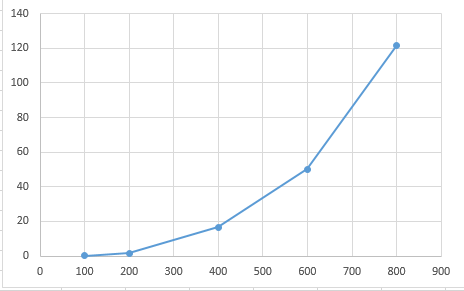
\includegraphics{genetic}

Zakładając stałą liczbę iteracji głównej pętli na złożoność składają się:

Krzyżowanie - pętla wykonywająca się tak długo aż dziecko będzie miało
wszystkie oligonukleotydy rodziców - liczba oligo w spektrum jest zależna
od n - długości dna, a także od temperatury. Wszystkie kroki w pętli mają
czas stały lub zależny liniowo od n np. znalezienie elementu w spektrum -
a więc ogólna złożoność funkcji jest kwadratowa.

Mutacje - liczba mutacji jest uzależniona od rozmiaru spektrum - złożoność liniowa. Wszystkie operacje występujące w funkcji mutacji również
mają koszt liniowy np. koszt znalezienia najgorszego elementu. Również i tutaj ogólna złożoność jest zależna od kwadratu z n.
           
Losowanie początkowej populacji, generowanie chwilowego rozwiązania mają złożoność liniową.

Wybranie najlepszych rodziców czyli de facto posortowanie całej populacji ma złożoność n*log(n) - stosujemy sortowanie szybkie - quicksort z biblioteki algorithm.

Co ciekawe wraz ze zwiększaniem temperatury rośnie, rośnie również czas wykonywania algorytmu co jest spowodowane trudniejszym dopasowywaniem oligonukleotydów do siebie - duży narzut ma tutaj krzyżowanie rodziców.

\section{Testy}

\section{Podsumowanie}

\end{document}

